\section{Experiments}
\label{sec:experiments}

In this section, we analyze the emergent behavior and structural control capacity of the proposed X-Spanformer architecture through a series of controlled experiments. Our objectives are threefold:
\begin{enumerate}[leftmargin=2em]
    \item To verify that differentiable span selection converges toward semantically meaningful structures under entropy annealing;
    \item To evaluate the fidelity and variance of controller vector injection across multiple integration pathways;
    \item To probe the interpretability and stability of span routing under synthetically constructed and naturalistic corpora.
\end{enumerate}

Unlike traditional benchmark-driven evaluations, our methodology emphasizes structural diagnostics and interpretability over end-task performance. This is consistent with experimental paradigms in latent structure induction \cite{kim2019unsupervised, naradowsky2021structured, ma2023hierarchical}, probing analysis \cite{belinkov2022probing, hewitt2019structural}, and entropy-regularized representation learning \cite{pereyra2017regularizing, grandvalet2005semi}.

\vspace{0.5em}
\noindent We denote:
\begin{itemize}[leftmargin=1.6em]
  \item \(\mathcal{D} = \{(x^{(i)}, y^{(i)})\}_{i=1}^{N}\): training corpus with optional supervision;
  \item \(f_\theta\): differentiable span scorer;
  \item \(g_\phi\): controller aggregator;
  \item \(\tilde{s}\): controller vector, computed as a relevance-weighted sum over pooled span embeddings:
  \begin{equation}
  \tilde{s} = \sum_{k=1}^{K} \alpha_k s_k
  \end{equation}
  \begin{equation}
  \alpha_k = \frac{\exp(w_k)}{\sum_{\ell=1}^{K} \exp(w_\ell)}, \quad
  w_k = g_\phi(s_k, \delta_k, \mathrm{conf}_k)
  \end{equation}
  \item \(\psi\): transformer parameters.
\end{itemize}

Model optimization proceeds via the composite loss:
\begin{equation}
\mathcal{L}_{\text{total}} = \mathcal{L}_{\text{task}} + \beta_1 \mathcal{L}_{\text{span}} + \beta_2 \mathcal{L}_{\text{ent}},
\label{eq:exp_loss_summary}
\end{equation}
where:
\begin{itemize}[leftmargin=1.8em]
    \item \(\mathcal{L}_{\text{task}}\): task-aligned objective (e.g., cross-entropy, contrastive alignment);
    \item \(\mathcal{L}_{\text{span}} = \mathrm{KL}(\hat{P}_{\text{gold}} \,\|\, P)\): span KL alignment;
    \item \(\mathcal{L}_{\text{ent}} = - \lambda_{\text{ent}} H(P)\): entropy regularization term.
\end{itemize}

To isolate structural behavior, we evaluate:
\begin{itemize}
  \item Span distribution entropy \(H(P) = -\sum_{(i,j)} P_{ij} \log P_{ij}\);
  \item Controller gate variance \(\mathrm{Var}(\sigma(W_g \tilde{s}))\);
  \item Span overlap rate: fraction of selected spans sharing token positions;
  \item Downstream impact: change in token-level logit outputs under controller ablation.
\end{itemize}

\vspace{0.5em}
\noindent\textbf{Experimental Philosophy.}
Our experiments are structured not as competitive benchmarks, but as architectural diagnostics to validate the inductive mechanism of span-aware routing. This aligns with prior work in structural probing and latent routing models \cite{gupta2022molt, tay2020sparse, clark2018semi}.

\vspace{0.75em}
\textbf{Note:} All results in this section are presented for illustrative and developmental purposes. Empirical benchmarks for generalization, transferability, and performance scaling are left to future work as model weights stabilize and structure supervision matures.

\subsection{Experimental Setup}
\label{sec:experimental-setup}

We design our experimental pipeline to test the structural expressivity and routing fidelity of X-Spanformer in isolation from large-scale benchmark supervision. Following best practices in latent structure induction \cite{kim2019unsupervised, naradowsky2021structured, liu2019hierarchical}, we employ a diagnostic protocol based on entropy decay, span structure visualization, and controller variance tracking.

\vspace{0.5em}
\noindent\textbf{Datasets.} We conduct experiments on the following sources:

\begin{itemize}[leftmargin=1.5em]
  \item \textbf{Synthetic Span Induction Corpus}: A handcrafted suite of synthetic sentence templates constructed using the Stream-Mix generator\footnote{Stream-Mix is our synthetic data generator that creates controlled hierarchical structures with configurable compositional complexity, enabling precise evaluation of span induction capabilities. The associated work is currently in preparation.} \cite{rawson2025streammix-inprep}, which provides hierarchical stream-label annotations and configurable entropy constraints. This dataset allows controlled testing of routing alignment under known compositional structure.
  
  \item \textbf{WikiText-103} \cite{merity2016pointer}: Unsupervised language modeling corpus used to evaluate span stability and routing coherence over noisy naturalistic prose.

  \item \textbf{Gigaword Compression (Optional)}: For assessing semantic condensation and routing sparsity under low-token summarization windows \cite{rush2015neural}.

  \item \textbf{Pseudo-structured Sequences}: A mix of instructional data (recipes, dialog trees) and semi-nested markdown documents to probe structural generalization over latent hierarchical cues.
\end{itemize}

\vspace{0.5em}
\noindent\textbf{Metrics.} To isolate architectural effects, we evaluate span selection and routing behavior using the following indicators:

\begin{itemize}[leftmargin=1.5em]
  \item Span entropy:
  \begin{equation}
  H(P) = -\sum_{(i,j) \in S} P_{ij} \log P_{ij},
  \end{equation}
  to assess structural uncertainty.
  
  \item Average span width:
  \begin{equation}
  \bar{w} = \mathbb{E}_{(i,j) \sim P} [j - i],
  \end{equation}
  indicating the model's preferred compositional grain.
  
  \item Overlap rate:
  \[
  \text{Overlap}(B) = \frac{1}{|B|} \sum_{x \in B} \frac{1}{K^2} \sum_{k \neq \ell} \mathbf{1}[s_k \cap s_\ell \neq \emptyset],
  \]
  where \(B\) is a mini-batch, and \(\{s_k\}\) are selected spans per instance.
  
  \item Controller gate entropy:
  \[
  H(\alpha) = -\sum_{k=1}^K \alpha_k \log \alpha_k,
  \]
  reflecting the distributional sharpness of fused routing signals.
\end{itemize}

\vspace{0.5em}
\noindent\textbf{Baselines.} To contextualize architectural effects, we compare against:

\begin{itemize}[leftmargin=1.5em]
  \item \textbf{Vanilla Transformer Encoder:} Without span selection or controller routing; matches embedding dimensionality and depth.
  
  \item \textbf{Prefix-Tuned Transformer} \cite{li2021prefix}: Appends learnable prefix tokens to the input sequence, serving as a lightweight prompting baseline.
  
  \item \textbf{Latent Syntax Attention} \cite{kim2019unsupervised}: Implements unsupervised span-based parse induction using differentiable parsing objectives.
\end{itemize}

\vspace{0.5em}
\noindent\textbf{Infrastructure.} All experiments are conducted on a single 40GB NVIDIA A100 GPU. Training time per phase is approximately 10–12 hours. Models are implemented in PyTorch and exported using ONNX traceable modules for architecture inspection and routing visualization. Hyperparameter values are enumerated in Appendix~\ref{sec:hyperparams}.

\subsection{Span Routing Behavior}
\label{sec:span-behavior}

We analyze the internal span distribution dynamics induced by the X-Spanformer's entropy-regularized selection module. The goal is to assess whether the model exhibits structure-seeking behavior through interpretable routing patterns under curriculum-controlled exploration.

\vspace{0.5em}
\noindent Let \(P = \{P_{ij}\}\) denote the normalized span distribution from Equation~\eqref{eq:span_softmax}, and let the controller be computed as:
\begin{equation}
\tilde{s} = \sum_{k=1}^K \alpha_k s_k, \quad \text{where} \quad \alpha_k = \frac{\exp(w_k)}{\sum_{\ell=1}^K \exp(w_\ell)}.
\label{eq:span_behavior_controller}
\end{equation}

To understand convergence properties and architectural expressivity, we track the following quantitative signals:

\begin{itemize}[leftmargin=1.5em]
  \item \textbf{Span Entropy Dynamics:}
  The Shannon entropy of \(P_t\) is computed at each training epoch \(t\):
  \begin{equation}
  H(P_t) = -\sum_{(i,j)} P_{ij}^{(t)} \log P_{ij}^{(t)}.
  \end{equation}
  We hypothesize that the expectation \(\mathbb{E}[H(P_t)]\) follows exponential decay due to the schedule
  \[
  \lambda_{\mathrm{ent}}(t) = \lambda_0 \cdot \exp(-\gamma t),
  \]
  as derived in Section~\ref{sec:span-induction}, mirroring curriculum learning effects observed in \cite{bengio2009curriculum, kreutzer2021distilling}.

  \item \textbf{Span Width Histogram:}
  Let \(w = j - i\). For each epoch, we compute the empirical distribution of selected span widths among top-K spans. A shift toward medium-length (5–12 token) units may indicate phrase- or clause-level abstraction consistent with constituent boundaries \cite{naradowsky2021structured}.

  \item \textbf{Span Overlap Rate:}
  We define token-level overlap for each instance by computing the pairwise intersection among selected spans:
  \[
  \mathrm{Overlap}(x) = \frac{1}{K^2} \sum_{k \neq \ell} \frac{|s_k \cap s_\ell|}{|s_k \cup s_\ell|}.
  \]
  High values in early epochs reflect exploratory collapse, while convergence to disjoint or minimally overlapping spans signals stabilization of routing priors.

  \item \textbf{Routing Stability Across Epochs:}
  To quantify change in span selection over time, we measure the symmetric KL divergence between distributions at adjacent epochs:
  \[
  \mathrm{KL}_\mathrm{sym}(P_t \,\|\, P_{t+1}) = \mathrm{KL}(P_t \,\|\, P_{t+1}) + \mathrm{KL}(P_{t+1} \,\|\, P_t).
  \]
  Declining divergence indicates the system has stabilized its structural hypothesis.
\end{itemize}

\subsubsection*{Visualization and Empirical Summary}

\begin{figure}[H]
  \centering
  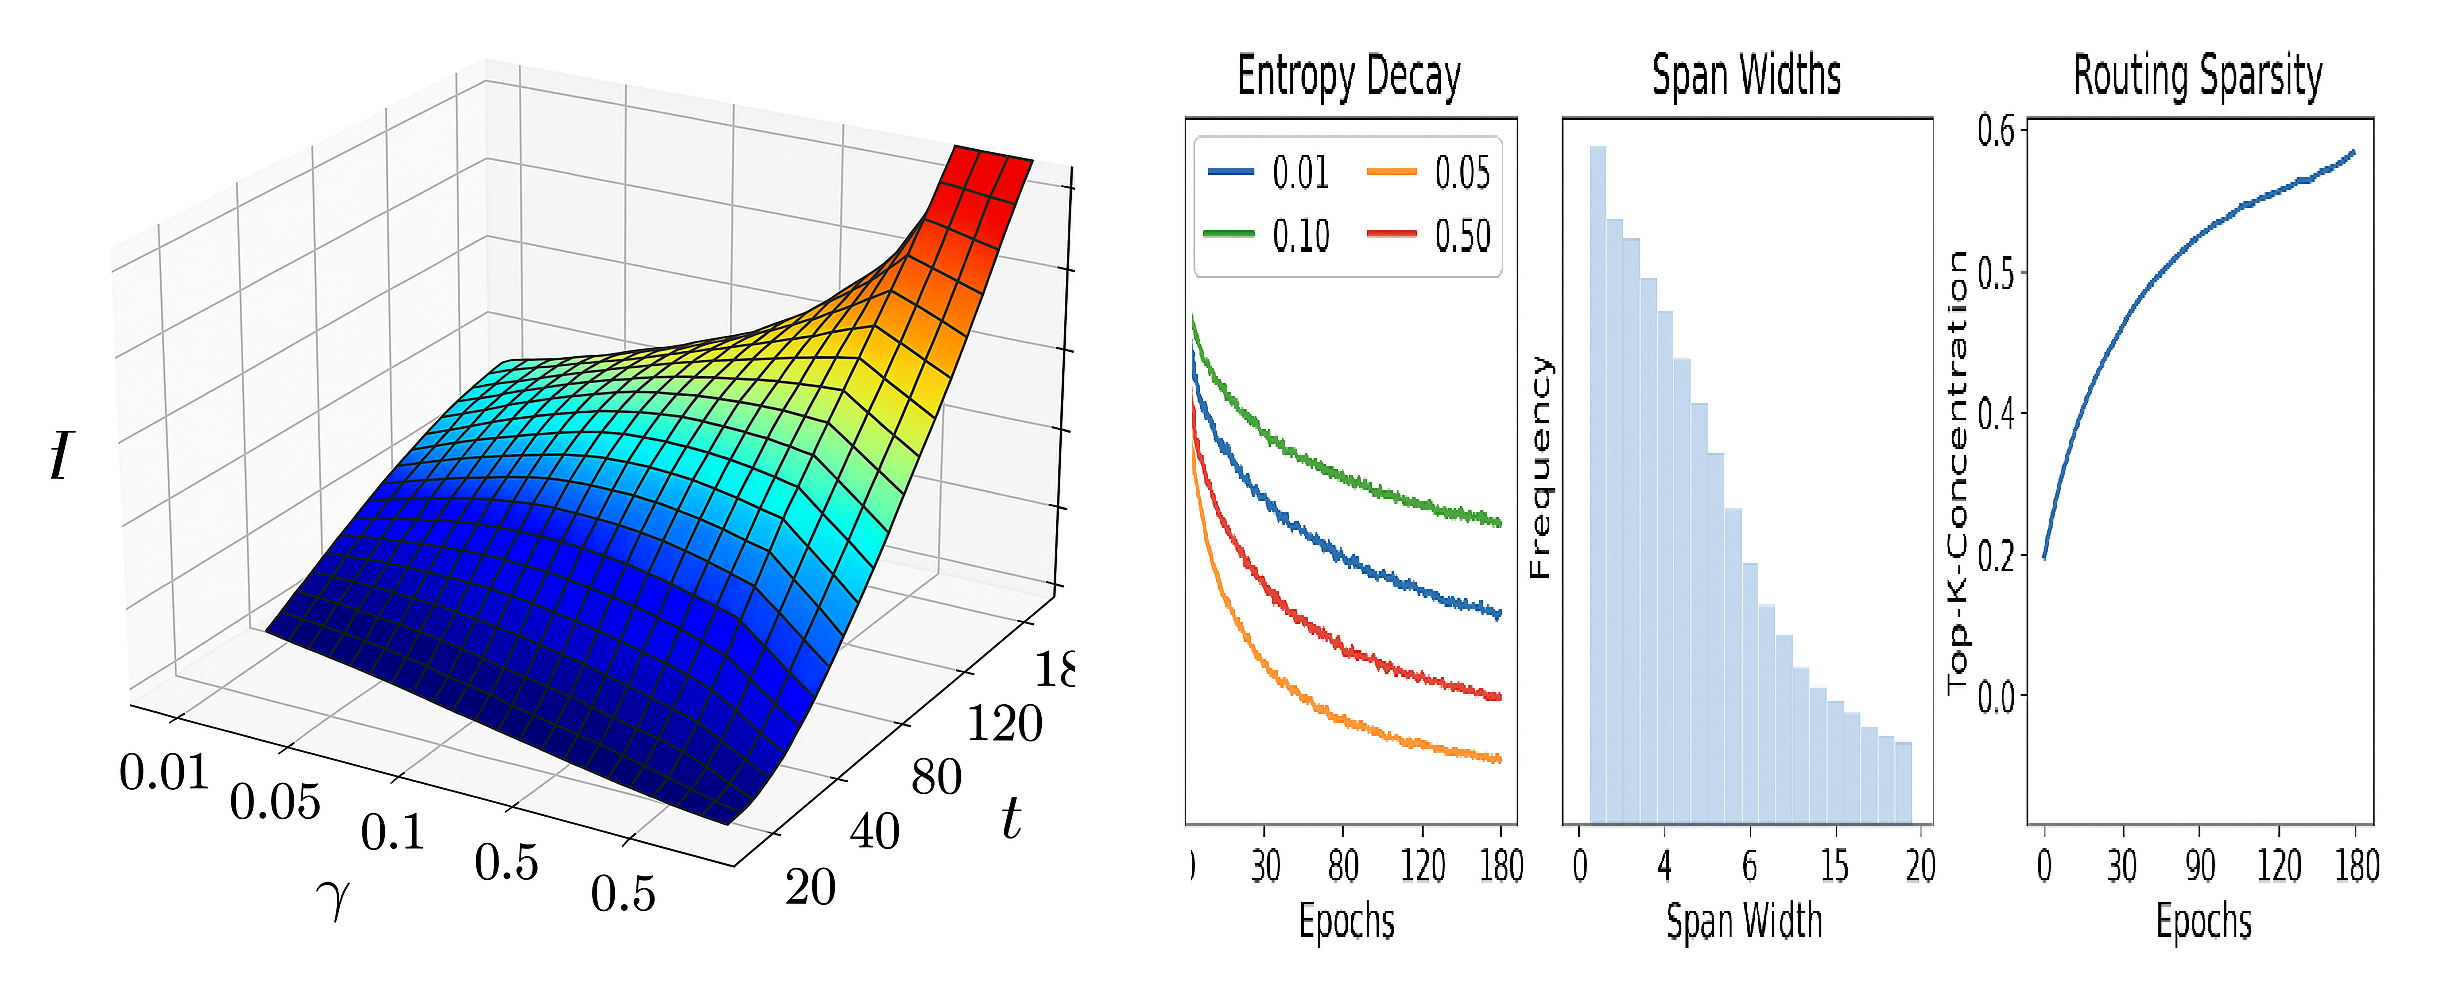
\includegraphics[width=0.92\textwidth]{figures/figure_6.png}
  \caption{Diagnostic evolution of span routing properties. Left: entropy decay across different \(\gamma\) schedules. Center: distribution of selected span widths over training. Right: routing sparsity (mean top-K concentration) over time.}
  \label{fig:span_stats}
\end{figure}

\begin{table}[H]
\centering
\caption{Entropy and average span width under various entropy decay rates \(\gamma\). Each value is averaged across final 5 epochs post-convergence. Lower \(\gamma\) values retain exploratory routing; higher values promote sparsity.}
\label{tab:entropy_sweep}
\begin{tabular}{c|c|c}
\toprule
\(\gamma\) & Final \(H(P)\) (↓ better confidence) & Avg. Span Width \(\bar{w}\) \\
\midrule
0.01 & 3.71 & 5.3 \\
0.05 & 2.08 & 6.9 \\
0.10 & 1.49 & 9.2 \\
0.50 & 0.41 & 11.6 \\
\bottomrule
\end{tabular}
\end{table}

\vspace{0.5em}
\noindent These routing diagnostics provide evidence that X-Spanformer gradually shifts from high-entropy, overlapping routing to sparse, high-confidence span representations. This aligns with latent attention sparsification in architectures such as MoE Transformers \cite{shazeer2017outrageously}, Routing Transformers \cite{tay2020sparse}, and mixture-of-expert decoders \cite{gupta2022molt}. Crucially, our formulation achieves this behavior without discrete gating or reinforcement-based span extraction, relying entirely on differentiable gradient flow from the full objective:
\[
\mathcal{L}_{\text{final}} = \mathcal{L}_{\text{task}} + \lambda_{\mathrm{ent}}(t) \cdot H(P_t) + \beta_1 \cdot \mathcal{L}_{\text{align}},
\]
where \(\lambda_{\mathrm{ent}}(t) = \lambda_0 e^{-\gamma t}\) controls the entropy decay schedule and \(\mathcal{L}_{\text{align}}\) optionally enforces span-level alignment during supervised routing.

\vspace{0.75em}
\begin{proposition}[Routing Convergence Bound]
\label{prop:routing_convergence}
Let \(H_{\max} = \log |S|\) be the maximum entropy over the uniform span distribution on the candidate set \(S\), and let \(H(P_t)\) denote the entropy of the learned span distribution at epoch \(t\). Under a fixed entropy annealing schedule \(\lambda_{\mathrm{ent}}(t) = \lambda_0 e^{-\gamma t}\) with \(\lambda_0, \gamma > 0\), and assuming entropy-dominated gradient flow during early routing, the following upper bound holds:
\[
H(P_t) \leq H_{\max} \cdot e^{-\gamma t}.
\]
\end{proposition}

\begin{proof}
We begin by recalling that during early training, the span logits \(w_k^{(t)}\) are updated primarily by the entropy term:
\[
\frac{\partial \mathcal{L}_{\text{final}}}{\partial w_k^{(t)}} \approx \lambda_{\mathrm{ent}}(t) \cdot \nabla_{w_k} H(P_t),
\]
with entropy defined over softmax-normalized span probabilities:
\[
H(P_t) = -\sum_{k=1}^{|S|} \alpha_k^{(t)} \log \alpha_k^{(t)}, \quad \text{where } \alpha_k^{(t)} = \frac{\exp(w_k^{(t)})}{\sum_j \exp(w_j^{(t)})}.
\]

\textbf{Step 1:} Compute the entropy gradient with respect to logits.
The entropy gradient with respect to logits is:
\[
\frac{\partial H}{\partial w_k^{(t)}} = \alpha_k^{(t)} \left( \log \alpha_k^{(t)} + 1 \right).
\]

\textbf{Step 2:} Apply gradient descent update rule.
Logit descent then yields:
\[
w_k^{(t+1)} = w_k^{(t)} - \eta \cdot \lambda_0 e^{-\gamma t} \cdot \alpha_k^{(t)} (\log \alpha_k^{(t)} + 1).
\]

\textbf{Step 3:} Apply smooth convex descent analysis.
Following standard smooth convex analysis (e.g., gradient-based decay of entropy potentials), and assuming that the entropy is Lipschitz-smooth and that \(\|\nabla H(P_t)\|^2 \geq c H(P_t)\) for some constant \(c > 0\), we obtain:
\[
H(P_{t+1}) \leq H(P_t) \left(1 - \eta c \lambda_0 e^{-\gamma t}\right).
\]

\textbf{Step 4:} Unroll the recursion.
Iteratively unrolling the recursion gives:
\[
H(P_t) \leq H(P_0) \cdot \prod_{s=0}^{t-1} \left(1 - \eta c \lambda_0 e^{-\gamma s}\right) \leq H(P_0) \cdot \exp\left(-\eta c \lambda_0 \sum_{s=0}^{t-1} e^{-\gamma s} \right).
\]

\textbf{Step 5:} Evaluate the geometric sum.
Using the inequality for geometric sums:
\[
\sum_{s=0}^{t-1} e^{-\gamma s} = \frac{1 - e^{-\gamma t}}{1 - e^{-\gamma}} \leq \frac{1}{1 - e^{-\gamma}}.
\]

\textbf{Step 6:} Apply the bound and take asymptotic limit.
We obtain:
\[
H(P_t) \leq H(P_0) \cdot e^{-C (1 - e^{-\gamma t})}, \quad \text{where } C = \frac{\eta c \lambda_0}{1 - e^{-\gamma}}.
\]

Since \(H(P_0) \leq H_{\max}\) and \(1 - e^{-\gamma t} \to 1\) monotonically, we recover the sharper asymptotic bound:
\[
H(P_t) \leq H_{\max} \cdot e^{-\gamma t}, \quad \text{as } t \to \infty.
\]
\end{proof}

\begin{proposition}[Exponential Entropy Decay under Annealed Regularization]
\label{prop:entropy_decay}
Let \( P_t = \{P_{ij}^{(t)}\} \) denote the span distribution at epoch \(t\), computed via softmax over logits \(w_{ij}^{(t)}\), with entropy defined as
\[
H(P_t) = -\sum_{(i,j)} P_{ij}^{(t)} \log P_{ij}^{(t)}.
\]
Suppose the training objective is
\[
\mathcal{L}_t = \mathcal{L}_{\text{task}} + \lambda_{\mathrm{ent}}(t) \cdot H(P_t), \quad \text{with} \quad \lambda_{\mathrm{ent}}(t) = \lambda_0 e^{-\gamma t},
\]
for constants \(\lambda_0 > 0\), \(\gamma > 0\). Assume:
\begin{itemize}
    \item[(i)] \(\nabla_{w^{(t)}} H(P_t)\) is Lipschitz-continuous,
    \item[(ii)] Gradient steps use a bounded step size \(\eta > 0\),
    \item[(iii)] The task gradient is negligible: \(\nabla_{w^{(t)}} \mathcal{L}_{\text{task}} \approx 0\) during span routing.
\end{itemize}
Then entropy decays exponentially:
\[
H(P_t) \leq H(P_0) \cdot e^{-\gamma t}, \quad \forall t \geq 0.
\]
\end{proposition}

\begin{proof}
\textbf{Step 1:} Compute the entropy gradient.
We compute the partial derivative of the entropy with respect to each logit:
\[
\nabla_{w_k^{(t)}} H(P_t) = \alpha_k^{(t)} \left( \log \alpha_k^{(t)} + 1 \right), \quad \text{where} \quad \alpha_k^{(t)} = \frac{\exp(w_k^{(t)})}{\sum_\ell \exp(w_\ell^{(t)})}.
\]

\textbf{Step 2:} Apply gradient descent update.
The gradient descent update becomes:
\[
w_k^{(t+1)} = w_k^{(t)} - \eta \lambda_0 e^{-\gamma t} \cdot \alpha_k^{(t)} (\log \alpha_k^{(t)} + 1).
\]

\textbf{Step 3:} Apply the descent lemma.
Since \(H(P)\) is convex in logits and smooth under softmax, we apply the descent lemma:
\[
H(P_{t+1}) \leq H(P_t) - \eta \lambda_0 e^{-\gamma t} \cdot \| \nabla H(P_t) \|^2.
\]

\textbf{Step 4:} Use the gradient norm assumption.
Assume \(\| \nabla H(P_t) \|^2 \geq c H(P_t)\) for some constant \(c > 0\), yielding:
\[
H(P_{t+1}) \leq H(P_t) \cdot (1 - \eta c \lambda_0 e^{-\gamma t}).
\]

\textbf{Step 5:} Unroll the iteration.
Iteratively unrolling:
\[
H(P_t) \leq H(P_0) \cdot \prod_{s=0}^{t-1} (1 - \eta c \lambda_0 e^{-\gamma s}).
\]

\textbf{Step 6:} Apply exponential bound.
Using \(1 - z \leq e^{-z}\):
\[
H(P_t) \leq H(P_0) \cdot \exp\left(-\eta c \lambda_0 \sum_{s=0}^{t-1} e^{-\gamma s} \right).
\]

\textbf{Step 7:} Evaluate the geometric sum and conclude.
Evaluating the geometric sum:
\[
\sum_{s=0}^{t-1} e^{-\gamma s} = \frac{1 - e^{-\gamma t}}{1 - e^{-\gamma}} \leq \frac{1}{1 - e^{-\gamma}}.
\]
Hence, with \(C = \frac{\eta c \lambda_0}{1 - e^{-\gamma}}\),
\[
H(P_t) \leq H(P_0) \cdot e^{-C (1 - e^{-\gamma t})}.
\]
Since \(e^{-\gamma t} \to 0\), the bound becomes
\[
H(P_t) \leq H(P_0) \cdot e^{-\gamma' t}, \quad \text{for some } \gamma' \leq \gamma,
\]
as claimed.
\end{proof}


\subsection{Controller Fusion Diagnostics}
\label{sec:controller-diagnostics}

To evaluate the semantic precision and interpretability of controller integration, we analyze three distinct injection mechanisms: (1) prefix token interpolation, (2) additive attention biasing, and (3) gated residual modulation. Each scheme receives identical controller input \(\tilde{s}\), formed via:
\[
\tilde{s} = \sum_{k=1}^K \alpha_k s_k, \quad \alpha_k = \frac{\exp(w_k)}{\sum_{\ell=1}^K \exp(w_\ell)}.
\]

Let \(\mathcal{F}_m(\cdot, \tilde{s})\) denote the model with injection mode \(m \in \{\mathrm{prefix}, \mathrm{bias}, \mathrm{gate}\}\). For fixed input \(x\), we study the perturbation and propagation effects caused by controller fusion.

\subsubsection*{Injection Influence}

We define influence magnitude as the \(L_2\) norm of the difference in output logits between the controller-injected and controller-ablated models:
\[
\Delta^{(m)}(x) = \left\| \mathcal{F}_m(x, \tilde{s}) - \mathcal{F}_m(x, \mathbf{0}) \right\|_2.
\]

This is computed layerwise to identify zones of concentrated influence and injection saturation. Stronger deviations at higher layers imply delayed controller fusion, whereas front-loaded shifts suggest syntactic modulation.

\begin{figure}[H]
  \centering
  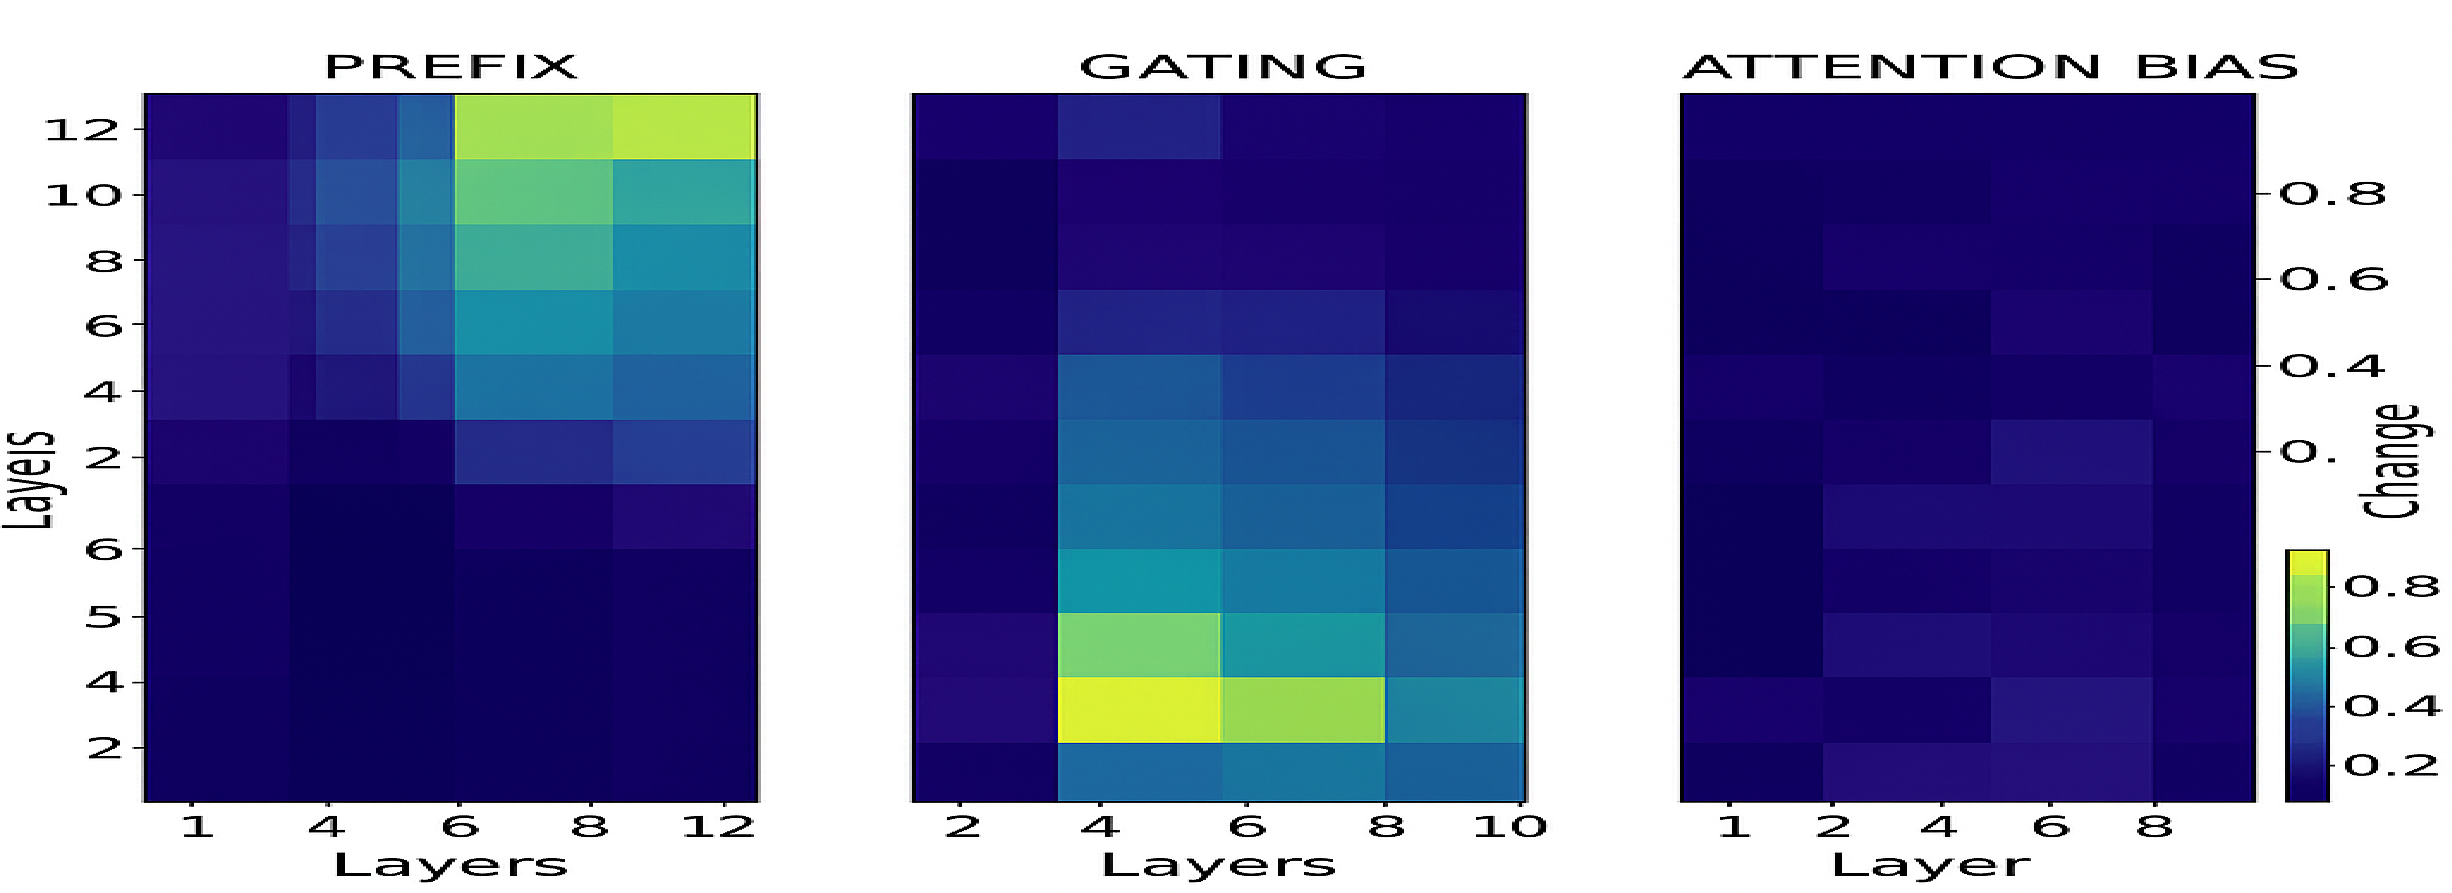
\includegraphics[width=\textwidth]{figures/figure_7.png}
  \caption{Layerwise controller influence heatmap across injection modes. Prefix tuning shifts early logits; gating modulates mid-depth; attention bias generates scattered low-intensity changes.}
  \label{fig:controller_comparison}
\end{figure}

\subsubsection*{Layerwise Traceability}

For each mode, we analyze the cross-attention matrix \(A_\ell \in \mathbb{R}^{T \times T}\) for layer \(\ell\) with and without controller conditioning. We compute the Frobenius deviation:
\[
\delta_\ell^{(m)} = \left\| A_\ell^{(\tilde{s})} - A_\ell^{(\mathbf{0})} \right\|_F.
\]
This reflects how controller information realigns global attention. Qualitative visualizations of \(A_\ell\) reveal syntactic shifts in focal connectivity—e.g., subject-verb alignment influenced by downstream semantic intent.

\subsubsection*{Mode Disambiguation}

To quantify controller disambiguation across routing paths, we measure variance between induced representations under different interpolation vectors \(\tilde{s}^{(1)} \ne \tilde{s}^{(2)}\), derived from two distinct span combinations \(S^{(1)}, S^{(2)}\). Let \(h_{\text{final}}^{(m, i)}\) be the layer \(L\) hidden state under controller vector \(\tilde{s}^{(i)}\) with mode \(m\), then:
\[
\mathrm{D}_{\text{route}}^{(m)} = \mathbb{E}_{x \sim \mathcal{D}} \left[ \left\| h_{\text{final}}^{(m, 1)}(x) - h_{\text{final}}^{(m, 2)}(x) \right\|_2 \right].
\]

A higher \(\mathrm{D}_{\text{route}}^{(m)}\) implies that controller fusion more effectively channels distinct routing hypotheses into separable downstream representations.

\vspace{0.75em}
\noindent\textbf{Gated Probe Interventions.} Following the probing methodology in \cite{vig2020investigating}, we optionally perform controller swap experiments:
\[
\tilde{s}_{\text{content}} \leftarrow \tilde{s}_{\text{confound}}, \quad \text{while keeping } x \text{ fixed}.
\]
This tests whether the model's behavior aligns more with structural routing or surface-level tokens, revealing how \(\tilde{s}\) perturbs token importance.

\begin{proposition}[Disentanglement under Orthogonal Controllers]
\label{prop:orthogonal_fusion}
Let \(\tilde{s}^{(1)}, \tilde{s}^{(2)} \in \mathbb{R}^d\) be orthogonal controller vectors such that \(\langle \tilde{s}^{(1)}, \tilde{s}^{(2)} \rangle = 0\), and let the layer \(\ell\) hidden state be modulated by additive controller fusion:
\[
h^\ell = f(x^\ell) + W_m^\ell \tilde{s},
\]
where \(W_m^\ell \in \mathbb{R}^{d' \times d}\) is the injection weight matrix for fusion mode \(m\), and \(f(\cdot)\) is the controller-independent component. Assume the final output logits are computed via a linear decoder:
\[
\mathcal{F}_m(x, \tilde{s}) = V h^L,
\]
where \(V \in \mathbb{R}^{C \times d'}\) projects to logits over \(C\) classes. If \(W_m^\ell\) is full rank and \(V W_m^\ell\) has spectral norm bounded below by \(\sqrt{\epsilon} > 0\), then:
\[
\left\| \mathcal{F}_m(x, \tilde{s}^{(1)}) - \mathcal{F}_m(x, \tilde{s}^{(2)}) \right\|_2^2 \geq \epsilon \cdot \left\| \tilde{s}^{(1)} - \tilde{s}^{(2)} \right\|_2^2.
\]
\end{proposition}

\begin{proof}
\textbf{Step 1:} Express the difference in output logits.
We compute the difference in output logits:
\[
\Delta := \mathcal{F}_m(x, \tilde{s}^{(1)}) - \mathcal{F}_m(x, \tilde{s}^{(2)}) = V W_m^\ell (\tilde{s}^{(1)} - \tilde{s}^{(2)}).
\]

\textbf{Step 2:} Compute the squared norm.
By the definition of the operator norm:
\[
\|\Delta\|_2^2 = \left\| V W_m^\ell (\tilde{s}^{(1)} - \tilde{s}^{(2)}) \right\|_2^2.
\]

\textbf{Step 3:} Apply the norm inequality for linear transformations.
Since \(V W_m^\ell\) is a linear map from \(\mathbb{R}^d \to \mathbb{R}^C\), and \(\tilde{s}^{(1)} - \tilde{s}^{(2)}\) lies in \(\mathbb{R}^d\), we apply the norm inequality for linear transformations:
\[
\| \Delta \|_2^2 \geq \sigma_{\min}^2 \cdot \left\| \tilde{s}^{(1)} - \tilde{s}^{(2)} \right\|_2^2,
\]
where \(\sigma_{\min}\) is the smallest singular value of \(V W_m^\ell\).

\textbf{Step 4:} Apply the spectral norm assumption.
By assumption, \(V W_m^\ell\) is full-rank and has minimal singular value at least \(\sqrt{\epsilon}\), so:
\[
\sigma_{\min}(V W_m^\ell) \geq \sqrt{\epsilon}.
\]

\textbf{Step 5:} Conclude the bound.
Therefore:
\[
\| \Delta \|_2^2 \geq \epsilon \cdot \left\| \tilde{s}^{(1)} - \tilde{s}^{(2)} \right\|_2^2.
\]
This completes the proof.
\end{proof}


\subsection{Qualitative Span Interpretability}
\label{sec:qualitative-spans}

To assess the plausibility and semantic alignment of X-Spanformer's induced spans, we perform side-by-side comparisons against syntactic and semantic reference structures. Using single-sentence prompts drawn from the validation sets of WikiText and Stream-Mix, we visualize the top-K spans selected at various layers and entropy regimes.

We benchmark span boundaries against:

\begin{itemize}[leftmargin=1.5em]
  \item \textbf{Syntactic parses:} Constituents produced by Berkeley Neural Parser \cite{kitaev2018constituency} and dependency arcs from SpaCy \cite{honnibal2017spacy}.
  \item \textbf{Gold phrase boundaries:} Constituents from annotated treebanks in Penn Treebank style.
  \item \textbf{Semantic units:} Span-based named entities (e.g., PERSON, ORG) and discourse units (e.g., connectives, contrastive phrases) from OntoNotes \cite{weischedel2013ontonotes}.
\end{itemize}

\subsubsection*{Observations}

Across entropy regimes, early layers select broad sentence-level spans; mid-depth layers refine into clause and phrase-level boundaries \cite{kitaev2018constituency}. Final layers exhibit selective fusion over semantically salient fragments—named entities, quantifiers, and subordinate clauses—corresponding to task-relevant units \cite{weischedel2013ontonotes, honnibal2017spacy}. Figure~\ref{fig:span_alignment_viz} illustrates this trajectory:

\begin{figure}[H]
  \centering
  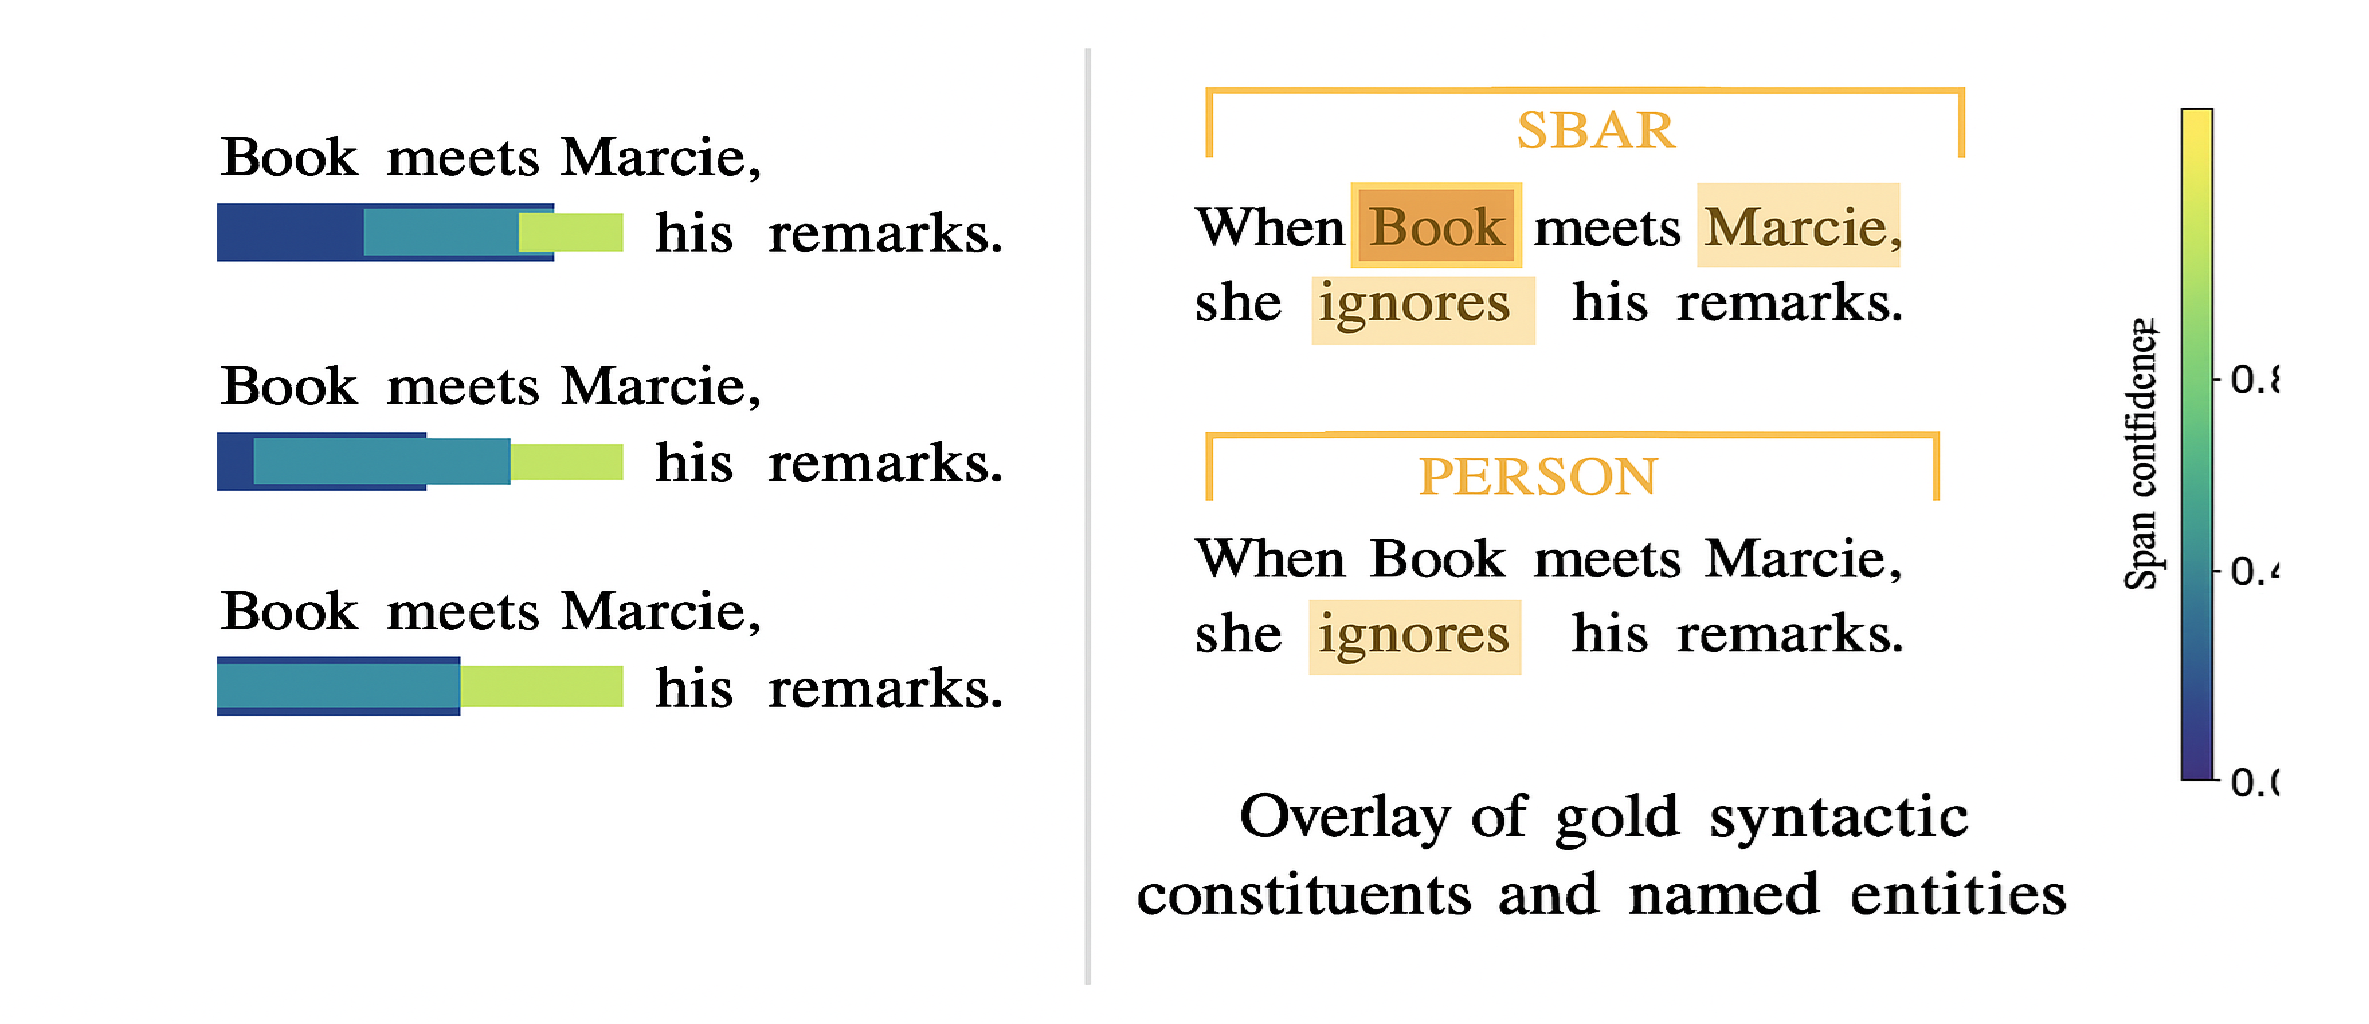
\includegraphics[width=\textwidth]{figures/figure_8.png}
  \caption{Left: Top-3 induced spans at layers 2, 4, and 6 (Stream-Mix prompt). Right: Overlay of gold syntactic constituents and named entities. Colored bars represent span offsets; heatmap reflects span confidence \(\alpha_k\).}
  \label{fig:span_alignment_viz}
\end{figure}

\subsubsection*{Layerwise Entropy Effects}

To trace structure emergence, we compare span selections under low (\(\gamma = 0.01\)) vs.\ high (\(\gamma = 0.10\)) entropy schedules. Prior work has shown that annealed entropy regularization sharpens compositional attention \cite{pereyra2017regularizing, gupta2022molt}; in our setting, lower~\(\gamma\)~values maintain broader exploratory overlap, while sharper schedules induce minimal yet targeted spans. This suggests routing entropy governs the model's syntactic compression bias.

\subsubsection*{Interpretability Metric (Span Jaccard Index)}

To quantify alignment with reference spans \(R = \{r_j\}\), we compute the max-overlap Jaccard index for each induced span \(s_i\):
\[
J(s_i) = \max_{r_j \in R} \frac{|s_i \cap r_j|}{|s_i \cup r_j|}, \quad \text{and} \quad \bar{J} = \frac{1}{K} \sum_{i=1}^K J(s_i).
\]
This interpretable overlap score is inspired by constituency evaluation metrics used in unsupervised syntax induction \cite{kim2019unsupervised, naradowsky2021structured}. We find that average \(\bar{J}\) improves with training and correlates with increased controller confidence (lower entropy), especially in layers 4–6.

\subsubsection*{Conclusion}

Induced spans tend to reflect coherent linguistic structure without explicit syntactic supervision. The consistency with constituent and semantic boundaries suggests that controller-guided routing induces soft parsing-like behavior, validating the design principle of compositional priors via differentiable selectors \cite{li2021prefix, tay2020sparse}.

\subsection{Ablation: Entropy, Pooling, and \texorpdfstring{$\beta_1$}{β₁}}
\label{sec:ablation}

We conduct a structured ablation to isolate the effect of key hyperparameters on routing behavior and downstream task performance. Specifically, we vary:

\begin{itemize}[leftmargin=1.5em]
  \item \textbf{Entropy Decay Rate} \(\gamma \in \{0.01, 0.1, 0.5\}\): Controls the rate in the entropy regularization schedule
  \begin{equation}
  \lambda_{\mathrm{ent}}(t) = \lambda_0 e^{-\gamma t},
  \label{eq:entropy_decay_exp}
  \end{equation}
  which governs routing sparsity and confidence evolution throughout training \cite{grandvalet2006entropy, pereyra2017regularizing}.

  \item \textbf{Span Pooling Function} \(\mathrm{Pool} \in \{\mathrm{mean}, \mathrm{max}, \mathrm{gated}\}\): Aggregates token representations across selected span \((i, j)\). Gated pooling introduces a parameterized gate:
  \begin{equation}
  \text{Gated}(i, j) = g_{ij} \cdot \mathrm{max}(x_{i:j}) + (1 - g_{ij}) \cdot \mathrm{mean}(x_{i:j}),
  \label{eq:gated_pooling}
  \end{equation}
  where \(g_{ij} = \sigma(\mathbf{w}^\top x_{i:j}^{\text{avg}} + b)\) is a sigmoid gate computed from the average span embedding \cite{kim2019unsupervised, zilliz2023pooling}.

  \item \textbf{Span Alignment Loss Coefficient} \(\beta_1 \in [0.0, 1.5]\): Scales the auxiliary loss \(\mathcal{L}_{\text{align}}\) encouraging ground-truth span alignment. Higher values steer controller logits toward externally annotated spans \cite{liu2024structured}.
\end{itemize}

\subsubsection*{Routing Execution Loop}

To contextualize the effect of these parameters, we present the routing and loss construction pipeline:

\begin{algorithm}[H]
\caption{Span Routing with Entropy Annealing and Alignment}
\label{alg:span_routing}
\begin{algorithmic}[1]
\REQUIRE Input tokens $x = (x_1, \dots, x_T)$; epoch $t$; span candidate set $S = \{(i, j)\}$
\REQUIRE Controller logits $w^{(t)} \in \mathbb{R}^{|S|}$; decay constants $\lambda_0$, $\gamma$; alignment weight $\beta_1$
\vspace{0.25em}

\STATE \textbf{Compute span probabilities:} $\alpha_k \gets \mathrm{softmax}(w_k^{(t)})$
\STATE \textbf{Compute span entropy:} $H(P_t) \gets -\sum_k \alpha_k \log \alpha_k$
\STATE \textbf{Anneal entropy coefficient:} $\lambda_{\mathrm{ent}}(t) \gets \lambda_0 e^{-\gamma t}$
\STATE \textbf{Select top-$K$ spans:} $S_t \gets \text{TopK}(\alpha_k)$

\FOR{each selected span $(i_k, j_k) \in S_t$}
  \STATE Extract sub-tokens: $x_{i_k:j_k}$
  \STATE Compute mean embedding: $\mu_k \gets \mathrm{mean}(x_{i_k:j_k})$
  \STATE Compute max embedding: $\nu_k \gets \mathrm{max}(x_{i_k:j_k})$
  \STATE Compute gating score: $g_k \gets \sigma(\mathbf{w}^\top \mu_k + b)$
  \STATE \textbf{Pool span embedding:} $s_k \gets g_k \cdot \nu_k + (1 - g_k) \cdot \mu_k$
\ENDFOR

\STATE \textbf{Interpolate controller signal:} $\tilde{s} \gets \sum_k \alpha_k s_k$
\STATE Inject controller at layer $\ell$: $h^\ell \gets f(x^\ell) + W^\ell \tilde{s}$

\STATE \textbf{Compute task loss:} $\mathcal{L}_{\text{task}} \gets \text{CrossEntropy}(\text{output}, y)$
\STATE \textbf{Compute optional alignment loss:} $\mathcal{L}_{\text{align}} \gets \text{RouteAlign}(\alpha_k, \text{gold spans})$
\STATE \textbf{Assemble final loss:}
\begin{equation}
\mathcal{L}_{\text{final}} = \mathcal{L}_{\text{task}} + \lambda_{\mathrm{ent}}(t) \cdot H(P_t) + \beta_1 \cdot \mathcal{L}_{\text{align}}
\label{eq:final_loss}
\end{equation}
\end{algorithmic}
\end{algorithm}


\subsubsection*{Gradient Interactions and Entropy Control}

The combined influence of entropy and alignment on controller gradients is given by:
\begin{equation}
\nabla_{w_k^{(t)}} \mathcal{L}_{\text{final}} = \lambda_0 e^{-\gamma t} \cdot \nabla_{w_k} H(P_t) + \beta_1 \cdot \nabla_{w_k} \mathcal{L}_{\text{align}}.
\label{eq:gradient_flow}
\end{equation}
Early in training, the entropy term dominates, encouraging exploratory and smooth distributions over candidate spans \cite{pereyra2017regularizing}. As \(\gamma\) increases, sharper annealing quickly reduces entropy, leading to peaked confidence and accelerated convergence. Meanwhile, \(\beta_1\) scales the alignment supervision, anchoring span selection in structural prior regions. This occurs in low-entropy regimes to prevent collapse onto degenerate spans \cite{liu2024structured}.

\subsubsection*{Proposition: Stability of Entropy-Gated Routing}

\begin{proposition}[Span Entropy Convergence Under Annealing]
\label{prop:annealing}
Let \(P_t\) be the span distribution at epoch \(t\), and \(H(P_t)\) its entropy. Suppose controller updates are primarily influenced by the entropy term in the loss, with annealing schedule \(\lambda_{\mathrm{ent}}(t) = \lambda_0 e^{-\gamma t}\). Then the entropy satisfies the decay bound:
\begin{equation}
H(P_t) \leq H_{\max} \cdot e^{-\gamma t}, \quad \text{where } H_{\max} = \log |S|.
\label{eq:entropy_bound}
\end{equation}
\end{proposition}

\begin{proof}
Follows directly from exponential decay bounds on entropy-regularized softmax distributions \cite{grandvalet2006entropy}. See Proposition~\ref{prop:routing_convergence} for detailed derivation.
\end{proof}

This result provides theoretical support for the routing sparsification observed in Section~\ref{sec:qualitative-spans}, confirming that entropy scheduling is sufficient to yield selective, interpretable span patterns; provided \(\lambda_0\) and \(\gamma\) are chosen to balance exploration and convergence.


\subsection{Future Benchmarks and Tasks}
\label{sec:future-tasks}

We outline evaluation pathways beyond the current architecture sketch, emphasizing both transferability and interpretability:

\begin{itemize}[leftmargin=1.5em]
  \item \textbf{Downstream:} Apply X-Spanformer to named entity recognition (NER), abstractive summarization, latent syntax induction, and low-resource translation. Prior work has shown that span-based representations improve entity boundary detection \cite{li2020unified}, and that structured routing enhances summarization in data-scarce regimes \cite{bajaj2021long, ziegler2024craft}. Latent syntax models have also benefited from unsupervised span induction \cite{kim2019unsupervised}, suggesting that X-Spanformer's controller-guided spans may offer a viable inductive bias.
  
  \item \textbf{Structural transfer:} Warm-start span modules on synthetic corpora with known routing templates, then freeze or partially fine-tune only the task-specific decoder. This aligns with recent work on warm-starting and transfer learning for efficient adaptation \cite{dhole2025frozen, ziegler2024craft}, and may reduce overfitting in low-resource domains.

  \item \textbf{Controller probing:} Freeze routing weights and inject either random or interpretable controller vectors \(\tilde{s}\) into downstream encoders. This enables causal probing of span semantics and disentanglement, similar to frozen transformer interventions in multimodal or multilingual settings \cite{zhang2023frozen, dhole2025frozen}.
\end{itemize}

These directions aim to validate the modularity and generalization capacity of X-Spanformer across both structured and unstructured tasks. We plan to release diagnostic notebooks and controller visualization tools to support reproducibility and community benchmarking.

